\documentclass[12pt,a4paper]{article}

% ─── Page Layout ───────────────────────────────────────────────────────────────
\usepackage[a4paper, margin=0.8in, headheight=14pt]{geometry}

% ─── Fonts (XeLaTeX) ───────────────────────────────────────────────────────────
\usepackage{fontspec}
\usepackage{unicode-math}
\setmainfont{TeX Gyre Pagella}
\setmonofont[Scale=0.88]{TeX Gyre Cursor}
\setmathfont{Latin Modern Math}

% ─── Packages ──────────────────────────────────────────────────────────────────
\usepackage{xcolor}
\usepackage{colortbl}
\usepackage{titlesec}
\usepackage{enumitem}
\usepackage{tabularx}
\usepackage{booktabs}
\usepackage{array}
\usepackage{amsmath}
\usepackage{tikz}
\usetikzlibrary{shapes.geometric, arrows.meta, positioning, calc, fit, decorations.pathreplacing}
\usepackage{tcolorbox}
\tcbuselibrary{skins, breakable}
\usepackage{hyperref}
\usepackage{fancyhdr}
\usepackage{graphicx}
\usepackage{microtype}
\hyphenpenalty=10000
\exhyphenpenalty=10000
\sloppy
\usepackage{caption}
\usepackage{setspace}
\usepackage{multirow}
\usepackage{tocloft}

% ─── Q&A helper ────────────────────────────────────────────────────────────────
\newcommand{\Q}[1]{\textbf{#1}\par\noindent\ignorespaces}

% ─── Colour Palette ────────────────────────────────────────────────────────────
\definecolor{myred}{RGB}{196,30,58}
\definecolor{mydark}{RGB}{30,30,50}
\definecolor{mygreen}{RGB}{14,120,80}
\definecolor{myteal}{RGB}{0,130,140}
\definecolor{myamber}{RGB}{180,100,0}
\definecolor{mypurple}{RGB}{100,30,160}
\definecolor{mygray}{RGB}{246,247,249}
\definecolor{mgframe}{RGB}{180,185,200}
\definecolor{watermark}{RGB}{145,150,170}
\definecolor{hdrred}{RGB}{250,232,235}
\definecolor{hdrgreen}{RGB}{220,244,233}
\definecolor{hdrteal}{RGB}{220,242,244}
\definecolor{hdramber}{RGB}{253,242,215}
\definecolor{hdrpurple}{RGB}{238,228,255}
\definecolor{hdrgray}{RGB}{238,240,245}
\definecolor{rowalt}{RGB}{250,251,253}

% ─── Section Formatting ────────────────────────────────────────────────────────
\titleformat{\section}
  {\large\bfseries\color{myred}}{\thesection.}{0.5em}{}
  [\vspace{1pt}{\color{myred}\rule{\linewidth}{0.8pt}}]
\titleformat{\subsection}
  {\normalsize\bfseries\color{myteal}}{\thesubsection}{0.5em}{}
\titlespacing*{\section}{0pt}{18pt}{7pt}
\titlespacing*{\subsection}{0pt}{11pt}{4pt}

% ─── Paragraph ─────────────────────────────────────────────────────────────────
\setlength{\parindent}{0pt}
\setlength{\parskip}{4pt}

% ─── TOC Styling ───────────────────────────────────────────────────────────────
\renewcommand{\cfttoctitlefont}{\large\bfseries\color{myred}}
\renewcommand{\cftaftertoctitle}{\par\noindent{\color{myred}\rule{\linewidth}{0.8pt}}}
\setlength{\cftbeforetoctitleskip}{0pt}
\setlength{\cftaftertoctitleskip}{6pt}
\renewcommand{\cftsecfont}{\normalsize\bfseries\color{mydark}}
\renewcommand{\cftsecpagefont}{\normalsize\bfseries\color{mydark}}
\renewcommand{\cftsecleader}{\cftdotfill{\cftdotsep}}
\setlength{\cftbeforesecskip}{7pt}
\renewcommand{\cftsubsecfont}{\small\color{mydark}}
\renewcommand{\cftsubsecpagefont}{\small\color{mydark}}
\setlength{\cftbeforesubsecskip}{3pt}
\setlength{\cftsubsecindent}{1.4em}

% ─── Table helpers ─────────────────────────────────────────────────────────────
\renewcommand{\arraystretch}{1.45}
\setlength{\tabcolsep}{6pt}
\arrayrulecolor{mydark}
\newcolumntype{B}[1]{>{\small\bfseries\raggedright\arraybackslash}m{#1}}
\newcolumntype{Y}{>{\small\raggedright\arraybackslash}X}
\renewcommand{\tabularxcolumn}[1]{m{#1}}

% ─── Header / Footer ───────────────────────────────────────────────────────────
\pagestyle{fancy}
\fancyhf{}
\fancyhead[L]{\small\color{myred}\textbf{PE-EC702B}\;\color{mydark}--- Digital Image and Video Processing}
\fancyhead[R]{\small\color{myteal}\textbf{Module 1 Notes}}
\fancyfoot[C]{\small\color{mydark}\thepage}
\fancyfoot[R]{\small\color{watermark}\textit{\copyright\ Biraj}}
\renewcommand{\headrulewidth}{0.5pt}
\renewcommand{\footrulewidth}{0.3pt}

% ─── Hyperref ──────────────────────────────────────────────────────────────────
\hypersetup{
  colorlinks=true, linkcolor=myteal, urlcolor=myteal,
  pdfauthor={Biraj Sarkar},
  pdftitle={PE-EC702B --- Module 1 Notes}
}

% ─── tcolorbox styles ──────────────────────────────────────────────────────────
\tcbset{
  tikzbox/.style={
    colback=mygray, colframe=mgframe, boxrule=0.6pt, arc=4pt,
    left=8pt, right=8pt, top=6pt, bottom=6pt,
    colbacktitle=mgframe, coltitle=mydark,
    fonttitle=\small\bfseries
  },
  defbox/.style={
    colback=hdrgreen, colframe=mygreen, boxrule=0.8pt, arc=4pt,
    left=9pt, right=9pt, top=6pt, bottom=6pt,
    colbacktitle=mygreen, coltitle=white,
    fonttitle=\small\bfseries
  },
  formulabox/.style={
    colback=hdrteal, colframe=myteal, boxrule=0.8pt, arc=4pt,
    left=9pt, right=9pt, top=7pt, bottom=7pt,
    colbacktitle=myteal, coltitle=white,
    fonttitle=\small\bfseries
  },
  examplebox/.style={
    colback=hdramber, colframe=myamber, boxrule=0.8pt, arc=4pt,
    left=9pt, right=9pt, top=6pt, bottom=6pt,
    colbacktitle=myamber, coltitle=white,
    fonttitle=\small\bfseries,
    breakable
  },
  masonbox/.style={
    colback=hdrpurple, colframe=mypurple, boxrule=0.8pt, arc=4pt,
    left=9pt, right=9pt, top=6pt, bottom=6pt,
    colbacktitle=mypurple, coltitle=white,
    fonttitle=\small\bfseries
  },
  exambox/.style={
    colback=hdrpurple, colframe=mypurple, boxrule=1pt, arc=5pt,
    left=10pt, right=10pt, top=8pt, bottom=8pt,
    colbacktitle=mypurple, coltitle=white,
    fonttitle=\bfseries,
    breakable, title after break={\textbf{Frequently Asked / Viva Questions (contd.)}}}
}
\tcbset{breakable}

% ─── TikZ styles ───────────────────────────────────────────────────────────────
\tikzset{
  block/.style={rectangle, draw=myteal, fill=hdrteal,
    text width=2.2cm, align=center, minimum height=0.85cm,
    font=\small, rounded corners=3pt, line width=0.7pt},
  arrow/.style={-Stealth, thick, color=mydark},
  redarrow/.style={-Stealth, thick, color=myred},
  line/.style={thick, color=mydark}
}

% ═══════════════════════════════════════════════════════════════════════════════
\begin{document}
% ═══════════════════════════════════════════════════════════════════════════════

\begin{center}
  {\LARGE\bfseries\color{myred} PE-EC702B --- Digital Image and Video Processing}\\[5pt]
  {\normalsize\color{mydark} Semester VII \quad$\bullet$\quad 3L:0T:0P \quad$\bullet$\quad 3 Credits}\\[3pt]
  {\normalsize\color{myteal}\textbf{Module 1 Exam Notes: Digital Image Fundamentals}}\\[3pt]
  {\small\color{mydark} CGEC \;$|$\; B.Tech ECE (2023--27) \;$|$\; \textit{Biraj Sarkar}}
\end{center}
\vspace{2pt}
\noindent{\color{myred}\rule{\linewidth}{1.5pt}}
\vspace{2pt}

\hypersetup{linkcolor=mydark}
\tableofcontents
\hypersetup{linkcolor=myteal}
\newpage

% ===============================================================================
\section{Elements of Visual Perception}
% ===============================================================================

Understanding human visual perception is crucial for digital image processing because the human eye is the ultimate receiver of the visual output.

\begin{tcolorbox}[defbox, title={Visual Perception Fundamentals}]
\textbf{Brightness Adaptation:} The human eye can operate over an enormous dynamic range ($10^{10}$ units), but cannot view this entire range simultaneously. It accomplishes this by changing its overall sensitivity, a process known as \textit{brightness adaptation}.
\end{tcolorbox}

\subsection{Eye Structure and Receptors}
The human eye contains two primary photoreceptors located on the retina:
\begin{itemize}[leftmargin=*, itemsep=2.5pt]
  \item \textbf{Cones (Photopic Vision):} Approximately 6 to 7 million receptors located mainly in the central portion of the retina (fovea). Highly sensitive to color. Allows resolve of fine details.
  \item \textbf{Rods (Scotopic Vision):} Approximately 75 to 150 million receptors distributed over the retinal surface. Give a general, overall picture of the field of view. Sensitive to low illumination levels (night vision), but are color-blind.
\end{itemize}

\subsection{Contrast Discrimination and Weber Ratio}
The ability of the eye to discriminate between different intensity levels is characterized by the \textbf{Weber Ratio}.
\begin{itemize}[leftmargin=*, itemsep=3pt]
  \item A subject is exposed to a uniform background intensity $I$.
  \item A short duration increment $\Delta I$ is added.
  \item The ratio $\frac{\Delta I}{I}$ at which the subject can just detect the change is called the \textbf{Weber Fraction}.
  \item A small Weber fraction indicates good intensity discrimination (high sensitivity), whereas a large fraction indicates poor discrimination (occurring at low illumination).
\end{itemize}

% ===============================================================================
\section{Image Sensing and Acquisition}
% ===============================================================================

To generate a digital image, the physical energy (light, X-ray, electromagnetic wave) must be converted into electrical signals by sensors.

\begin{tcolorbox}[defbox, title={Image Sensor Configurations}]
\textbf{Image Sensors:} Devices that convert illumination energy into electrical voltage. There are three primary configurations:
\begin{enumerate}[label=(\alph*), leftmargin=*, itemsep=1pt]
  \item \textbf{Single Sensor:} Uses a photodiode that moves mechanically in $x$- and $y$-directions (e.g., microdensitometers).
  \item \textbf{Sensor Strips:} Inline array of sensors providing 1D line scans (e.g., flatbed scanners).
  \item \textbf{Sensor Array:} 2D grid of sensors capturing the entire scene (e.g., CCD/CMOS arrays in digital cameras).
\end{enumerate}
\end{tcolorbox}

% ===============================================================================
\section{Image Sampling and Quantization}
% ===============================================================================

A continuous image $f(x,y)$ must be converted into digital format in both spatial coordinates (sampling) and amplitude (quantization).

\begin{tcolorbox}[defbox, title={Sampling vs. Quantization}]
\textbf{Sampling:} Digitizing the continuous spatial coordinates $(x,y)$ into discrete grid indices.
\par\noindent
\textbf{Quantization:} Digitizing the continuous amplitude (intensity values) into discrete gray levels.
\end{tcolorbox}

\subsection{Representing Digital Images}
A digital image of size $M \times N$ with $L$ discrete gray levels is represented as a matrix:
\begin{equation}
  f(x,y) = \begin{bmatrix}
    f(0,0) & f(0,1) & \cdots & f(0,N-1) \\
    f(1,0) & f(1,1) & \cdots & f(1,N-1) \\
    \vdots & \vdots & \ddots & \vdots \\
    f(M-1,0) & f(M-1,1) & \cdots & f(M-1,N-1)
  \end{bmatrix}
\end{equation}
The number of gray levels $L$ is typically a power of 2:
\begin{equation}
  L = 2^k
\end{equation}
where $k$ is the number of bits required to store each pixel. The total number of bits $b$ required to store the image is:
\begin{equation}
  b = M \times N \times k
\end{equation}

\subsection{Resolution and Spatial Regressions}
\begin{itemize}[leftmargin=*, itemsep=3.5pt]
  \item \textbf{Spatial Resolution:} The smallest discernible detail in an image, measured in dots/pixels per unit distance (e.g., dpi). Insufficient spatial sampling causes \textbf{aliasing} (moir\'{e} patterns).
  \item \textbf{Intensity Resolution:} The smallest discernible change in gray level, measured in bits per pixel.
  \item \textbf{False Contouring:} An effect caused by insufficient quantization levels (typically $k < 4$ bits), producing visible, artificial boundaries between smooth gray-level transitions.
\end{itemize}

% ===============================================================================
\section{Basic Relationships Between Pixels}
% ===============================================================================

Let $p$ and $q$ be pixels in an image. Their relationships determine boundaries, regions, and structures.

\subsection{Pixel Neighborhoods}
\begin{itemize}[leftmargin=*, itemsep=3.5pt]
  \item \textbf{4-neighbors ($N_4(p)$):} The 4 horizontal and vertical pixels adjacent to $p$ at coordinates:
    \begin{equation}
      (x+1, y), \quad (x-1, y), \quad (x, y+1), \quad (x, y-1)
    \end{equation}
  \item \textbf{Diagonal neighbors ($N_D(p)$):} The 4 diagonal pixels adjacent to $p$ at coordinates:
    \begin{equation}
      (x+1, y+1), \quad (x+1, y-1), \quad (x-1, y+1), \quad (x-1, y-1)
    \end{equation}
  \item \textbf{8-neighbors ($N_8(p)$):} The union of 4-neighbors and diagonal neighbors:
    \begin{equation}
      N_8(p) = N_4(p) \cup N_D(p)
    \end{equation}
\end{itemize}

\subsection{Adjacency and Path Connectivity}
Let $V$ be the set of intensity values used to define adjacency (e.g., $V = \{1\}$ in binary images, or $V = \{128, \dots, 255\}$ in grayscale).
\begin{enumerate}[leftmargin=*, itemsep=3.5pt]
  \item \textbf{4-adjacency:} Two pixels $p$ and $q$ with values in $V$ are 4-adjacent if $q \in N_4(p)$.
  \item \textbf{8-adjacency:} Two pixels $p$ and $q$ with values in $V$ are 8-adjacent if $q \in N_8(p)$.
  \item \textbf{m-adjacency (mixed adjacency):} Two pixels $p$ and $q$ with values in $V$ are m-adjacent if:
    \begin{itemize}[leftmargin=1.5em, itemsep=1pt]
      \item $q \in N_4(p)$, OR
      \item $q \in N_D(p)$ and the intersection $N_4(p) \cap N_4(q)$ has no pixels with values from $V$.
    \end{itemize}
    \textit{Purpose: m-adjacency is introduced to eliminate the multiple path ambiguities that arise in 8-adjacency.}
\end{enumerate}

\begin{tcolorbox}[tikzbox, title={Pixel Neighborhoods and m-Adjacency}]
\centering
\begin{minipage}{0.45\textwidth}
  \centering
  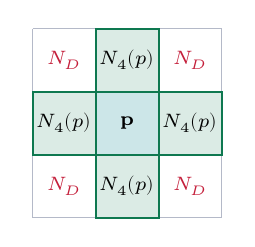
\begin{tikzpicture}[scale=0.8, every node/.style={font=\scriptsize}]
    % Neighbor Grid
    \draw[step=1.0cm, color=mgframe, line width=0.6pt] (0,0) grid (3,3);
    
    % Center pixel p
    \fill[color=myteal!20, draw=myteal, line width=0.8pt] (1,1) rectangle (2,2);
    \node at (1.5, 1.5) {\textbf{p}};
    
    % 4-neighbors
    \fill[color=mygreen!15, draw=mygreen, line width=0.7pt] (1,2) rectangle (2,3); \node at (1.5,2.5) {$N_4(p)$};
    \fill[color=mygreen!15, draw=mygreen, line width=0.7pt] (1,0) rectangle (2,1); \node at (1.5,0.5) {$N_4(p)$};
    \fill[color=mygreen!15, draw=mygreen, line width=0.7pt] (2,1) rectangle (3,2); \node at (2.5,1.5) {$N_4(p)$};
    \fill[color=mygreen!15, draw=mygreen, line width=0.7pt] (0,1) rectangle (1,2); \node at (0.5,1.5) {$N_4(p)$};
    
    % Diagonal neighbors
    \node[color=myred] at (0.5,2.5) {\textbf{$N_D$}};
    \node[color=myred] at (2.5,2.5) {\textbf{$N_D$}};
    \node[color=myred] at (0.5,0.5) {\textbf{$N_D$}};
    \node[color=myred] at (2.5,0.5) {\textbf{$N_D$}};
  \end{tikzpicture}
  \par\vspace{2pt}\small\textbf{Pixel Neighbors}
\end{minipage}
\hfill
\begin{minipage}{0.48\textwidth}
  \centering
  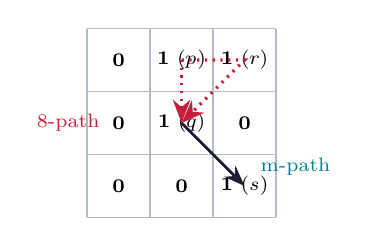
\begin{tikzpicture}[scale=0.8, every node/.style={font=\scriptsize}]
    % 8-path vs m-path grid
    \draw[step=1.0cm, color=mgframe, line width=0.6pt] (0,0) grid (3,3);
    
    \node at (0.5, 2.5) {\textbf{0}};
    \node at (1.5, 2.5) {\textbf{1} ($p$)};
    \node at (2.5, 2.5) {\textbf{1} ($r$)};
    
    \node at (0.5, 1.5) {\textbf{0}};
    \node at (1.5, 1.5) {\textbf{1} ($q$)};
    \node at (2.5, 1.5) {\textbf{0}};
    
    \node at (0.5, 0.5) {\textbf{0}};
    \node at (1.5, 0.5) {\textbf{0}};
    \node at (2.5, 0.5) {\textbf{1} ($s$)};

    % Draw paths
    \draw[redarrow, dotted, line width=1.2pt] (1.5, 2.5) -- (2.5, 2.5) -- (1.5, 1.5);
    \draw[redarrow, dotted, line width=1.2pt] (1.5, 2.5) -- (1.5, 1.5);
    \node[color=myred] at (-0.3, 1.5) {8-path};
    
    % m-path
    \draw[arrow, line width=1pt] (1.5, 1.5) -- (2.5, 0.5);
    \node[color=myteal, right] at (2.6, 0.8) {m-path};
  \end{tikzpicture}
  \par\vspace{2pt}\small\textbf{m-path resolves 8-path ambiguity}
\end{minipage}
\end{tcolorbox}

\subsection{Distance Measures}
Let $p(x,y)$, $q(s,t)$, and $z(v,w)$ be pixels. A distance function $D(p,q)$ must satisfy:
\begin{itemize}[leftmargin=*, itemsep=2pt]
  \item $D(p,q) \ge 0$ ($D(p,q) = 0$ if and only if $p = q$)
  \item $D(p,q) = D(q,p)$ (Symmetry)
  \item $D(p,z) \le D(p,q) + D(q,z)$ (Triangle Inequality)
\end{itemize}

\begin{tcolorbox}[formulabox, title={Key Distance Metrics}]
\textbf{Euclidean Distance ($D_e$):}
\begin{equation}
  D_e(p,q) = \sqrt{(x-s)^2 + (y-t)^2}
\end{equation}
\par\noindent
\textbf{City-Block Distance ($D_4$):}
\begin{equation}
  D_4(p,q) = |x-s| + |y-t|
\end{equation}
\par\noindent
\textbf{Chessboard Distance ($D_8$):}
\begin{equation}
  D_8(p,q) = \max(|x-s|, |y-t|)
\end{equation}
\end{tcolorbox}

% ===============================================================================
\section{Worked Examples}
% ===============================================================================

\begin{tcolorbox}[examplebox, title={Distance Calculations and Path Analysis}]
\textbf{Problem:} Given pixel $p$ at coordinates $(3,4)$ and pixel $q$ at coordinates $(7,8)$ in a digital image:
\begin{enumerate}[label=(\alph*), leftmargin=*, itemsep=2pt]
  \item Calculate the Euclidean distance $D_e(p,q)$.
  \item Calculate the City-Block distance $D_4(p,q)$.
  \item Calculate the Chessboard distance $D_8(p,q)$.
  \item Determine if there is an m-path between $p$ and $q$ using $V = \{1\}$ in the following $3 \times 3$ grid segment, where the coordinates are:
  \begin{center}
    \begin{tabular}{c c c}
      $a(0,2) = 0$ & $b(1,2) = 1$ & $c(2,2) = 1$ \\
      $d(0,1) = 0$ & $e(1,1) = 1$ & $f(2,1) = 0$ \\
      $g(0,0) = 0$ & $h(1,0) = 0$ & $i(2,0) = 1$
    \end{tabular}
  \end{center}
\end{enumerate}

\par\noindent\rule{\linewidth}{0.5pt}\par
\textbf{Solution:}
\par\noindent
\textbf{(a) Euclidean Distance ($D_e$):}
\begin{equation*}
  D_e(p,q) = \sqrt{(3-7)^2 + (4-8)^2} = \sqrt{(-4)^2 + (-4)^2} = \sqrt{16+16} = \sqrt{32} \approx 5.66
\end{equation*}

\textbf{(b) City-Block Distance ($D_4$):}
\begin{equation*}
  D_4(p,q) = |3-7| + |4-8| = 4 + 4 = 8
\end{equation*}

\textbf{(c) Chessboard Distance ($D_8$):}
\begin{equation*}
  D_8(p,q) = \max(|3-7|, |4-8|) = \max(4, 4) = 4
\end{equation*}

\textbf{(d) m-path Analysis:}
\begin{itemize}[leftmargin=*, itemsep=2pt]
  \item We seek a path of pixels with value $1$ between $e(1,1)$ and $i(2,0)$ under m-adjacency rules.
  \item Let's check neighbors of $e(1,1)$:
    \begin{itemize}[leftmargin=1em, itemsep=1.5pt]
      \item $b(1,2)$ has value $1$ and is a 4-neighbor of $e$ ($b \in N_4(e)$). Thus, there is an m-path segment $e \leftrightarrow b$.
      \item $i(2,0)$ is a diagonal neighbor of $e$ ($i \in N_D(e)$).
      \item Under m-adjacency rules, diagonal pixels $e$ and $i$ are m-adjacent only if the intersection of their 4-neighbors has no pixels of value $V=\{1\}$.
      \item $N_4(e) \cap N_4(i) = \{ (2,1), (1,0) \} = \{ f, h \}$.
      \item Since $f(2,1) = 0$ and $h(1,0) = 0$, both intersection pixels have value $0$, which is not in $V$.
      \item Therefore, $e$ and $i$ are directly m-adjacent. The path is $e \leftrightarrow i$ (length 1).
    \end{itemize}
  \item Now let's check path from $b(1,2)$ to $i(2,0)$:
    \begin{itemize}[leftmargin=1em, itemsep=1.5pt]
      \item $c(2,2)$ is in $N_4(b)$ and has value $1$. Thus, $b \leftrightarrow c$.
      \item $i(2,0)$ is a diagonal neighbor of $f$, but $c$ and $i$ are not adjacent. The only valid path is $b \leftrightarrow e \leftrightarrow i$.
    \end{itemize}
\end{itemize}
\end{tcolorbox}

\newpage

% ===============================================================================
% MANDATORY QUICK REVISION PAGE
% ===============================================================================
\begin{center}
  {\large\bfseries\color{myred} Quick Revision --- Module I}\\[3pt]
  {\small\color{mydark} Digital Image Fundamentals $|$ PE-EC702B}
\end{center}
\noindent{\color{myred}\rule{\linewidth}{1.2pt}}
\vspace{4pt}

\begin{tcolorbox}[formulabox, title={\textbf{Key Formulas at a Glance}}]
\renewcommand{\arraystretch}{1.3}
\begin{tabularx}{\linewidth}{B{5.0cm} X}
Quantization Levels & $L = 2^k$ \quad ($k$ = bit depth) \\
Storage Requirement & $b = M \times N \times k$ \quad (bits for an $M \times N$ image) \\
Euclidean Distance & $D_e(p,q) = \sqrt{(x-s)^2 + (y-t)^2}$ \\
City-Block Distance & $D_4(p,q) = |x-s| + |y-t|$ \\
Chessboard Distance & $D_8(p,q) = \max(|x-s|, |y-t|)$ \\
Weber Fraction & $\text{Weber Ratio} = \frac{\Delta I}{I}$ \quad ($\Delta I$ = just noticeable increment)
\end{tabularx}
\end{tcolorbox}

\begin{tcolorbox}[defbox, title={\textbf{One-Line Definitions}}]
\begin{itemize}[leftmargin=*, itemsep=2.5pt, topsep=0pt]
  \item \textbf{Photopic Vision:} Vision mediated by cone cells under bright light, providing high color and spatial resolution.
  \item \textbf{Scotopic Vision:} Vision mediated by rod cells under low light, providing color-blind, coarse spatial vision.
  \item \textbf{Sampling:} Discretizing continuous coordinates $(x,y)$ to define spatial resolution.
  \item \textbf{Quantization:} Discretizing continuous amplitude (gray level) to define intensity resolution.
  \item \textbf{False Contouring:} Artificial banding appearing in regions of smooth transitions due to low quantization.
  \item \textbf{m-Adjacency:} Mixed adjacency that prevents dual-path ambiguities by checking vertical/horizontal neighbors.
\end{itemize}
\end{tcolorbox}

\begin{tcolorbox}[exambox, title={\textbf{Frequently Asked / Viva Questions}}]
\begin{enumerate}[leftmargin=*, itemsep=3.5pt, label=\arabic*.]
  \item \Q{State the difference between rods and cones.} Cones are located mainly in the fovea, are color-sensitive, and operate in bright light (photopic vision). Rods are distributed across the retina, are highly sensitive to low light (scotopic vision), and are color-blind.
  \item \Q{What is Weber ratio? What does a low Weber ratio imply?} It is the ratio of the just noticeable increment in intensity $\Delta I$ to the background intensity $I$. A low Weber ratio implies high intensity discrimination capability of the human eye.
  \item \Q{Why is m-adjacency preferred over 8-adjacency?} 8-adjacency can lead to multiple, ambiguous paths between two pixels (e.g., both diagonal and horizontal-vertical paths simultaneously). m-adjacency resolves this by choosing the diagonal path only when no horizontal-vertical path exists.
  \item \Q{Explain the concept of false contouring.} If the number of quantization levels $L$ is too low (typically $< 16$ levels), the smooth transitions of intensity appear as discrete, nested bands of constant gray level with sharp, artificial boundaries.
  \item \Q{How does city-block distance differ from chessboard distance?} $D_4$ distance (city-block) allows only horizontal and vertical movements, while $D_8$ distance (chessboard) allows both horizontal-vertical and diagonal movements. For any two points, $D_8(p,q) \le D_4(p,q)$.
  \item \Q{What is spatial resolution and how is it measured?} It is the smallest discernible detail in an image. It is measured in terms of line pairs per unit distance or dots per inch (dpi).
  \item \Q{What is the storage size of a $512 \times 512$ image with 256 gray levels?} $256 = 2^8$, so $k = 8$ bits. Total size $b = 512 \times 512 \times 8 = 2,097,152 \text{ bits} = 256 \text{ KB}$.
  \item \Q{What causes aliasing in digital images?} Aliasing occurs when the sampling frequency is less than twice the maximum spatial frequency of the image (violating the Nyquist criterion), causing high-frequency details to wrap as moir\'{e} patterns.
  \item \Q{Define a path between two pixels $p$ and $q$.} A path is a sequence of distinct pixels $(x_0, y_0), (x_1, y_1), \dots, (x_n, y_n)$ where $(x_0, y_0) = p$, $(x_n, y_n) = q$, and $(x_i, y_i)$ is adjacent to $(x_{i-1}, y_{i-1})$ for all $1 \le i \le n$.
  \item \Q{What are the components of an image sensing device?} An image sensing device consists of a filter (to select wavelength band), a sensing material (to convert photon energy to charge), and a readout circuit (to convert charge to voltage).
\end{enumerate}
\tcbset{colbacktitle=myteal, coltitle=white}
\end{tcolorbox}

\begin{tcolorbox}[tikzbox, title={Comparison of Pixel Distances}]
\centering
\renewcommand{\arraystretch}{1.2}
\begin{tabularx}{\linewidth}{>{\bfseries}B{3.5cm} Y Y}
\rowcolor{hdrgray} Distance Metric & Path allowed & Value for $p(0,0)$ and $q(2,2)$ \\
\midrule
Euclidean ($D_e$) & Straight line (any angle) & $\sqrt{2^2 + 2^2} = \sqrt{8} \approx 2.83$ \\
\rowcolor{rowalt} City-Block ($D_4$) & Horizontal and vertical only & $2 + 2 = 4$ \\
Chessboard ($D_8$) & Horizontal, vertical, and diagonal & $\max(2,2) = 2$ \\
\bottomrule
\end{tabularx}
\end{tcolorbox}

\end{document}
